\chapter{SYSTEM DESIGN}
\thispagestyle{empty}

This chapter describes the system architecture, the module decomposition of
the API, the database design, the security architecture, and the key
workflows of the platform.

\clearpage

\section{System Architecture}

The system is a modular monolith deployed as a single Docker Compose stack.
The public boundary is a Cloudflare Tunnel; all traffic flows through it to
an internal nginx reverse proxy, which routes the web application and the API
on their path prefixes. Internal services (PostgreSQL, RabbitMQ, the OCR
service, the workers, the AI gateway) are reachable only over the private
Docker network. Figure~\ref{fig:arch} shows the deployment topology.

\begin{figure}[H]
\centering
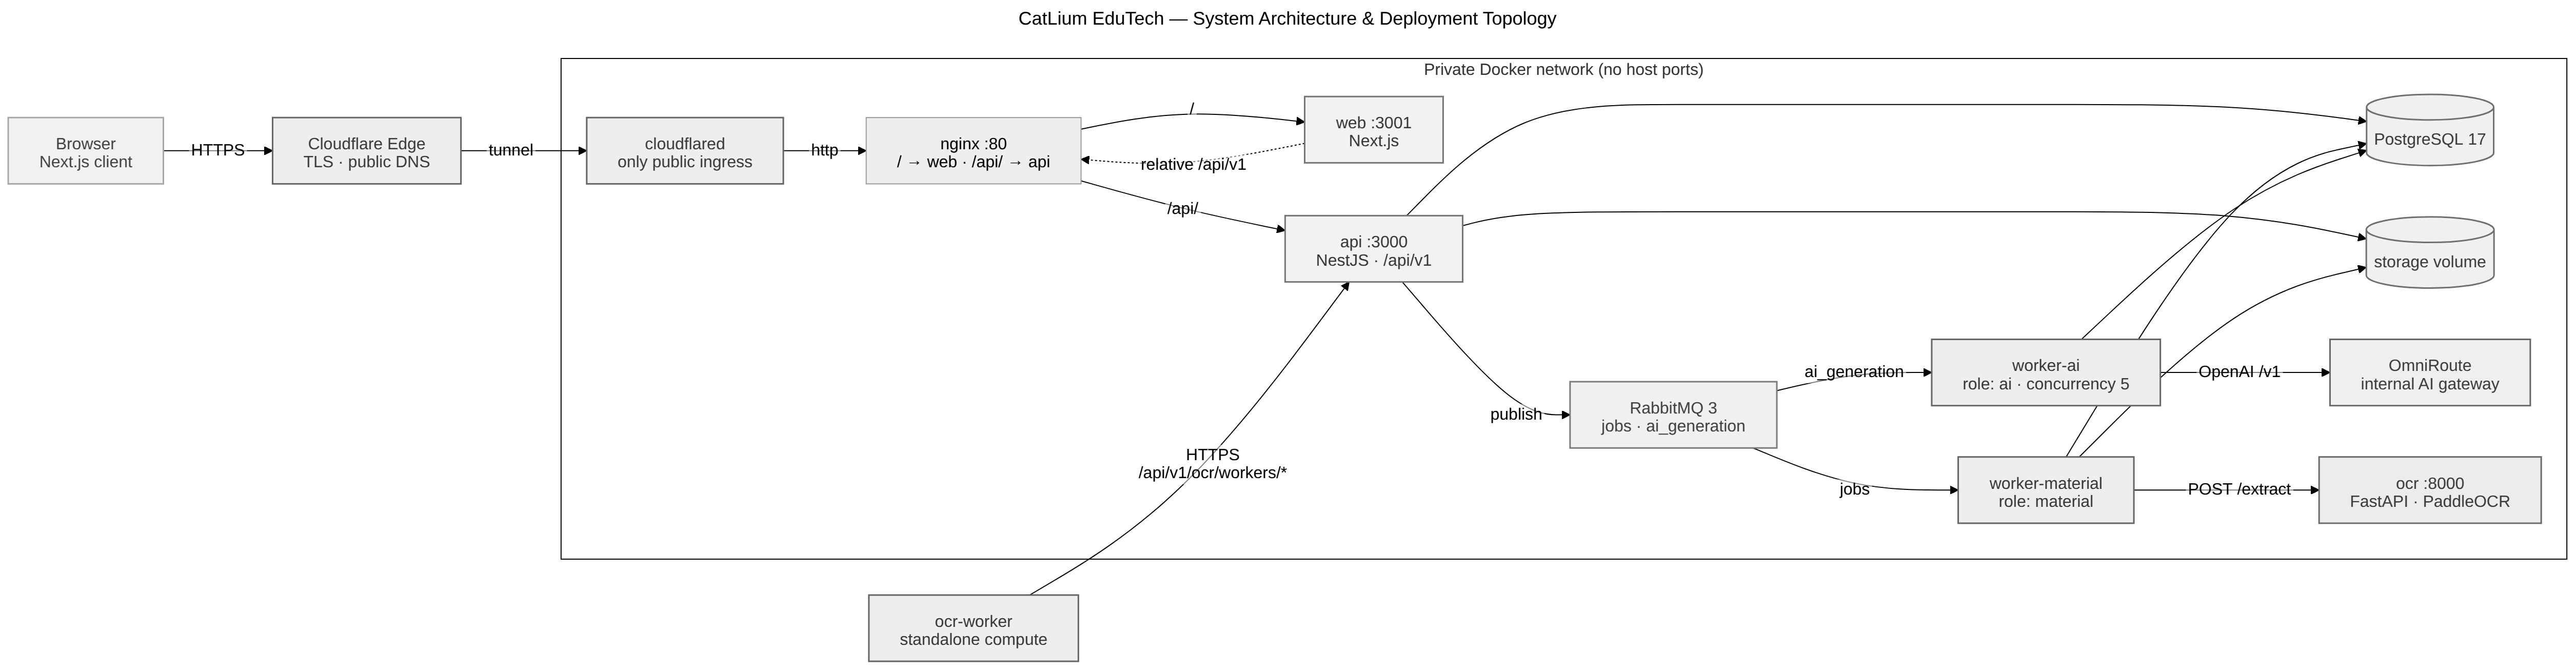
\includegraphics[width=\textwidth]{figures/system-architecture-bw.png}
\caption{System architecture and deployment topology. The Cloudflare Tunnel
is the only public ingress; nginx routes to the Next.js web app and the
NestJS API, and all other services are internal to the private network.}
\label{fig:arch}
\end{figure}

Asynchronous work is distributed over RabbitMQ with two queues: a general
\texttt{jobs} queue consumed by the material worker and an
\texttt{ai\_generation} queue consumed by the AI worker. The API publishes
job messages and tracks job lifecycle in the database; it never executes
heavy work itself.

\section{Module Architecture}

The API is organised into bounded modules (Table~\ref{tab:modules}).
Flashcards, notes, and Cornell notes are not separate modules: they are study
content types stored in the content module and governed by type-specific
payload contracts.

\begin{table}[H]
\centering
\caption{API domain modules and their responsibilities.}
\label{tab:modules}
\small
\begin{tabular}{@{}l p{\dimexpr\textwidth-3.6cm-12pt\relax}@{}}
\toprule
\textbf{Module} & \textbf{Responsibility} \\
\midrule
identity & Cookie-based login, refresh, logout, current user \\
tenancy & Institute membership lookup and role derivation \\
users & Institute user management and status control \\
jobs & Asynchronous job register, queue publication, retry, cancel \\
academic & Subjects, chapters, topics with soft delete and restore \\
content & Versioned study content items and AI generation \\
materials & Material upload, OCR processing, page inspection \\
ocr & Distributed OCR coordination and worker registry \\
material-enhancement & Cleaning, structuring, segmentation, syllabus mapping \\
questions & Question bank, batches, review, AI generation \\
question-extraction & Deterministic extraction of question candidates \\
paper-patterns & Pattern structure, validation, approval, extraction \\
question-papers & Paper authoring, pattern selection, assembly \\
examinations & Assessments, scope, publication, per-assessment questions \\
syllabus & Syllabus upload, OCR, AI analysis, confirmation \\
attempts & Attempt snapshots, evaluation, results, analytics \\
practice & Ungraded flashcard and question practice \\
export & DOCX, PDF, and spreadsheet export with previews \\
health & Readiness endpoint \\
\bottomrule
\end{tabular}
\end{table}

\section{Deployment Architecture}

\textsc{cloudflared}, the tunnel client, is the only component that maps the
deployment to a public hostname. nginx binds inside the private network and
routes \texttt{/} to the web application and \texttt{/api/} to the NestJS
API with the prefix preserved. PostgreSQL, Redis, RabbitMQ, the OCR service,
the workers, and OmniRoute are declared in the compose stack without host
ports in the production posture. A development override exposes loopback-only
ports for local tooling. The OCR service also supports a standalone worker
model in which additional devices claim page-range chunks from the API over
HTTP.

\section{Database Design}

The database is PostgreSQL 17 managed with Drizzle ORM and uses JSONB for
flexible structured payloads (content payloads, pattern structures, progress
records). Thirty-three tables cover the domains in
Table~\ref{tab:entities}. All domain tables carry an institute reference or
are otherwise tenant-scoped, and scope chains are enforced by check
constraints (a topic belongs to a chapter which belongs to a subject).
Figure~\ref{fig:erd} shows the full entity--relationship diagram.

\begin{table}[H]
\centering
\caption{Database entity groups in the schema.}
\label{tab:entities}
\small
\begin{tabular}{@{}p{3.6cm} p{\dimexpr\textwidth-3.6cm-12pt\relax}@{}}
\toprule
\textbf{Group} & \textbf{Tables} \\
\midrule
Identity \& tenancy & users, auth\_sessions, institutes, memberships, membership\_roles \\
Academic & subjects, chapters, topics \\
Content & content\_items, content\_versions \\
Materials \& OCR & materials, ocr\_workers, ocr\_chunks, ocr\_page\_corrections \\
Material Intelligence & material\_enhancements, material\_enhancement\_segments, material\_enhancement\_segment\_mappings \\
Questions & questions, question\_types \\
Papers & question\_papers, question\_paper\_questions, paper\_patterns, paper\_pattern\_subjects \\
Examinations & assessments, assessment\_questions \\
Attempts & attempts, attempt\_questions, attempt\_responses \\
Practice & practice\_sessions, practice\_session\_items, practice\_session\_responses \\
Syllabus & syllabi \\
Jobs & jobs \\
\bottomrule
\end{tabular}
\end{table}

\begin{figure}[H]
\centering
\includegraphics[width=\textwidth]{figures/database-erd-bw.png}
\caption{Entity--relationship diagram of the PostgreSQL schema.}
\label{fig:erd}
\end{figure}

\section{Security Architecture}

Authentication uses an access JWT stored in an httpOnly cookie plus a
refresh cookie; the refresh token is stored hashed in \texttt{auth\_sessions}
and rotated on every refresh with concurrency handling. State-changing
requests verify a CSRF double-submit token. On every request the guard stack
runs in order: the access-token guard, the tenant guard (which validates
the \texttt{x-institute-id} header against an active membership), and the
roles guard. Figure~\ref{fig:auth} shows the sequence. Internal services
authenticate with an \texttt{x-internal-api-key} header, and student-facing
payloads are sanitized so that answer keys and explanations never leave the
API.

\begin{figure}[H]
\centering
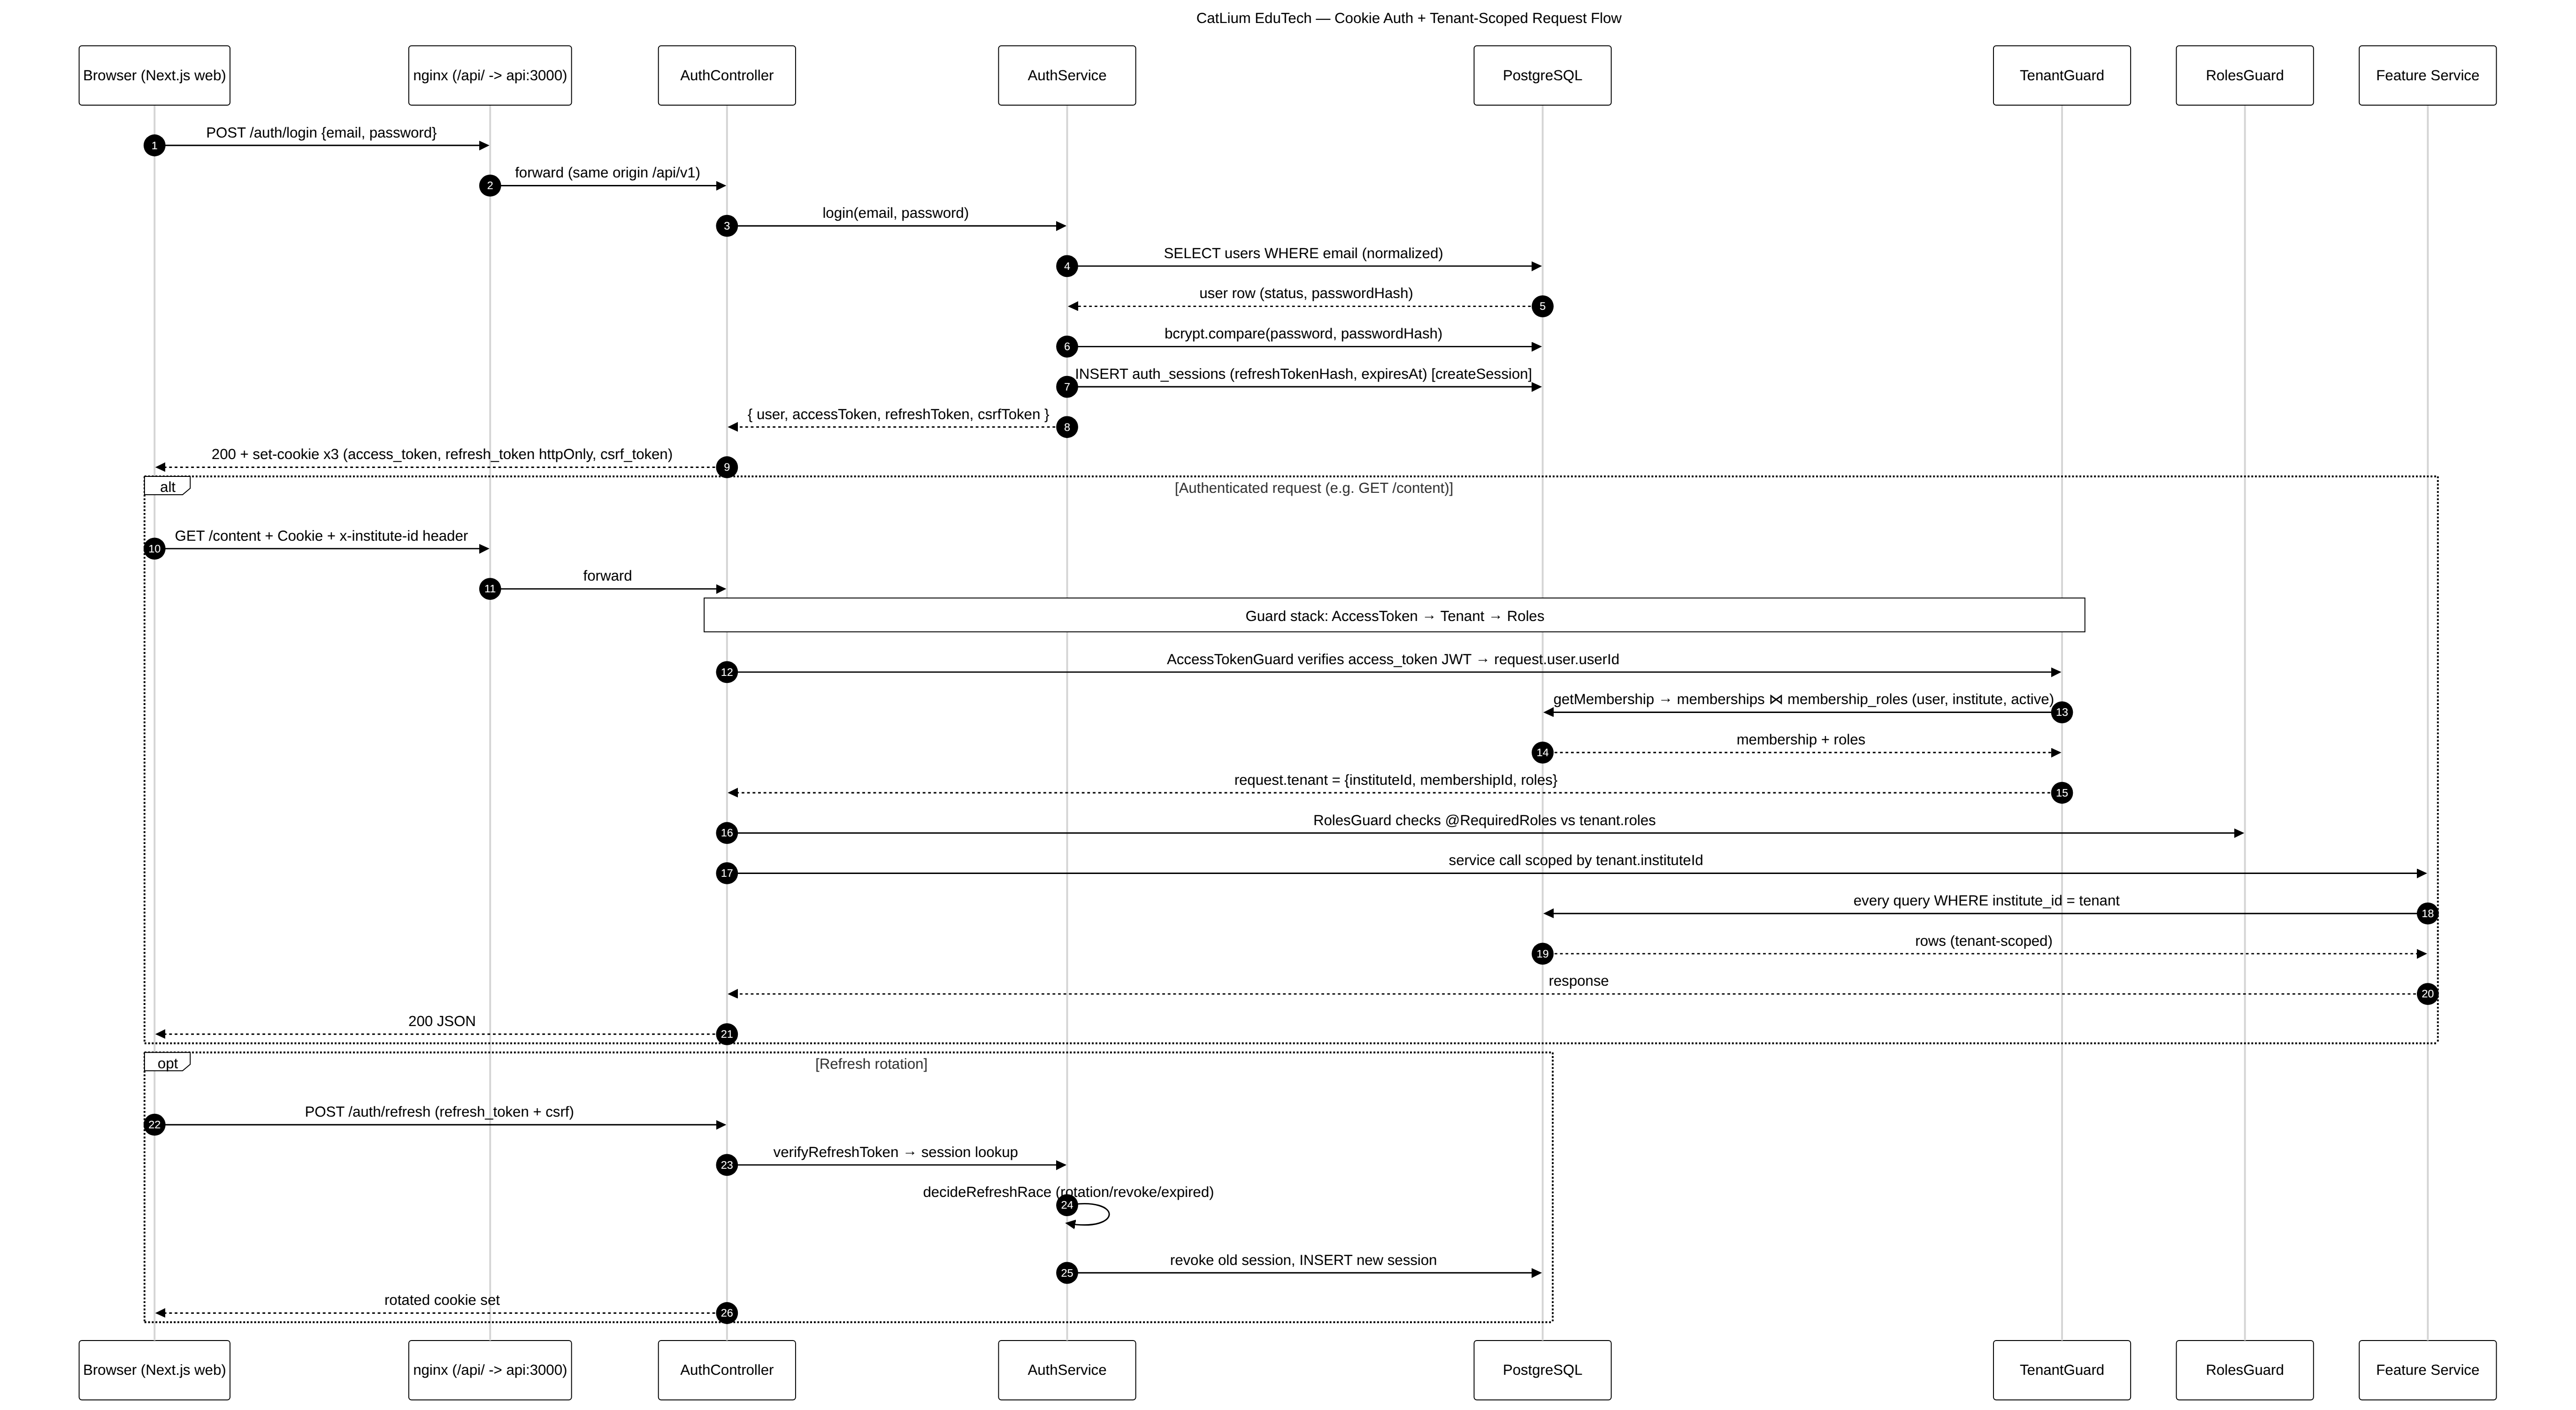
\includegraphics[width=\textwidth]{figures/authentication-sequence-bw.png}
\caption{Authentication and per-request authorization sequence.}
\label{fig:auth}
\end{figure}

\section{Key Workflows}

\subsection{Distributed OCR processing}

Materials are processed in an OCR pipeline with page-level fidelity. PDF
pages with embedded text are extracted directly; pages without text fall
back to PaddleOCR. Processing is distributed: an API-side coordinator
materializes page-range chunks, workers (local or standalone) claim chunks,
extract their page ranges, and submit results; a periodic sweep settles
timed-out work. Figure~\ref{fig:ocr} shows the sequence, and
Figure~\ref{fig:ocrstate} the chunk and job lifecycles.

\begin{figure}[H]
\centering
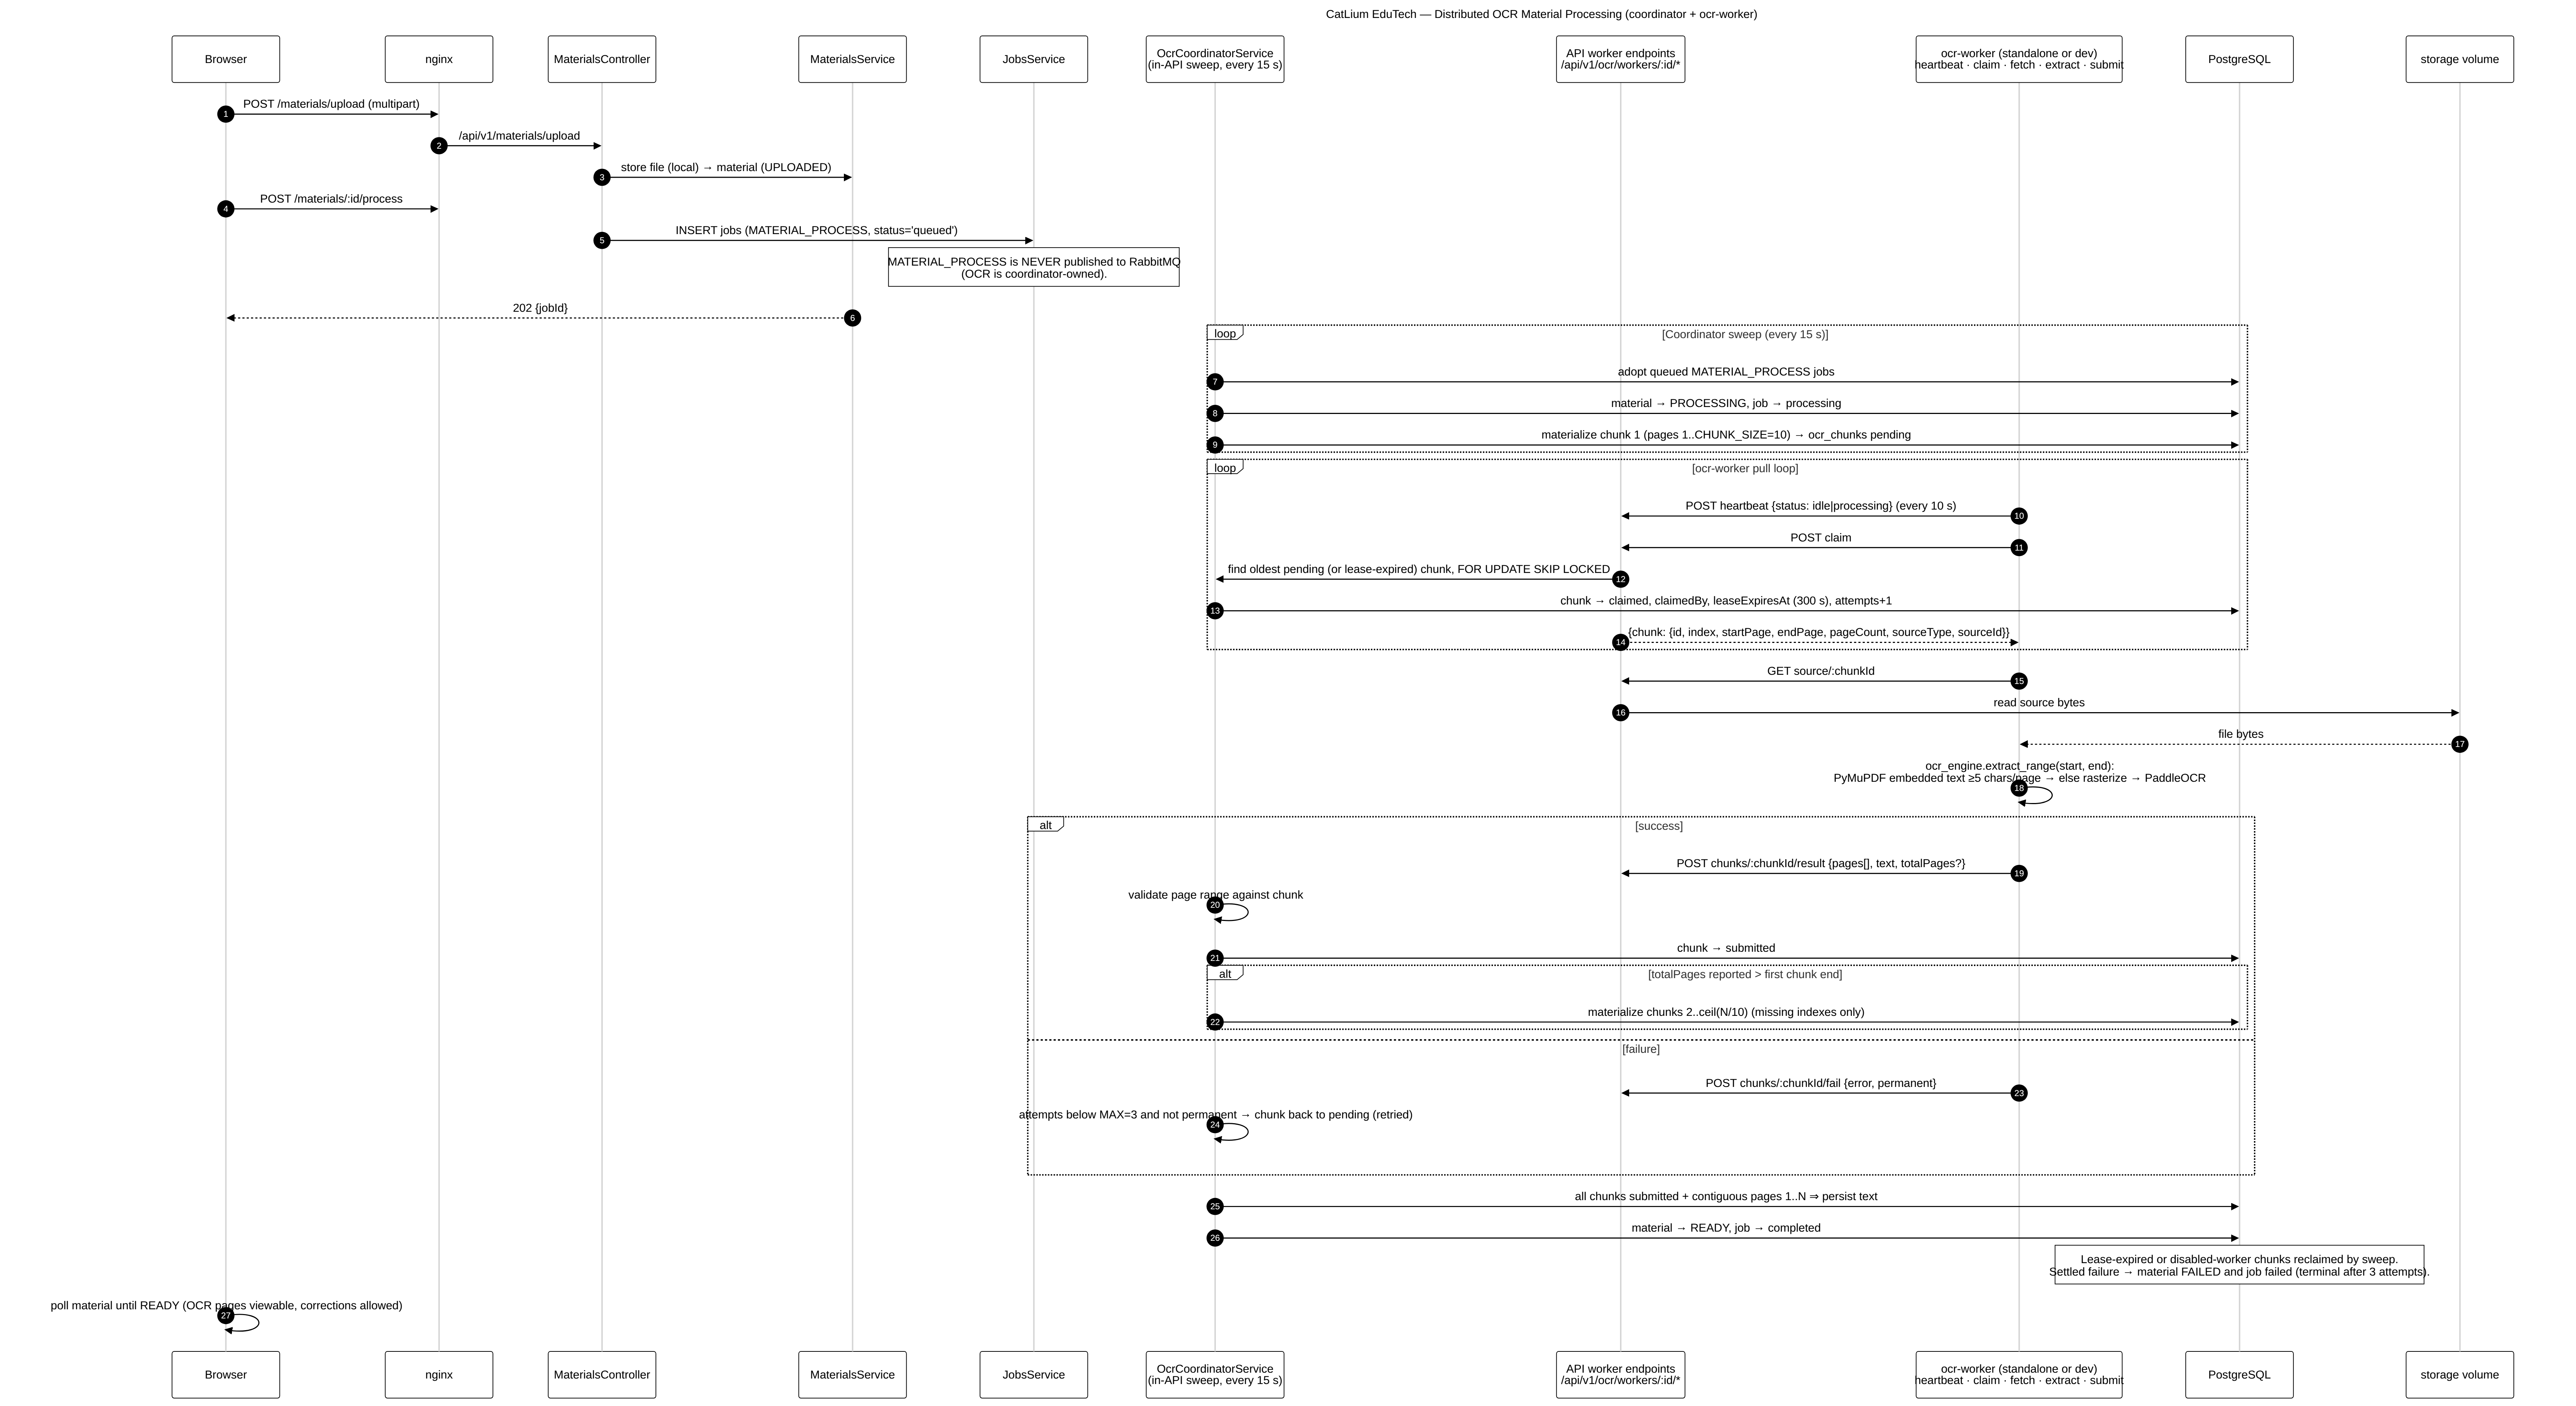
\includegraphics[width=\textwidth]{figures/ocr-processing-sequence-bw.png}
\caption{Distributed OCR processing sequence.}
\label{fig:ocr}
\end{figure}

\begin{figure}[H]
\centering
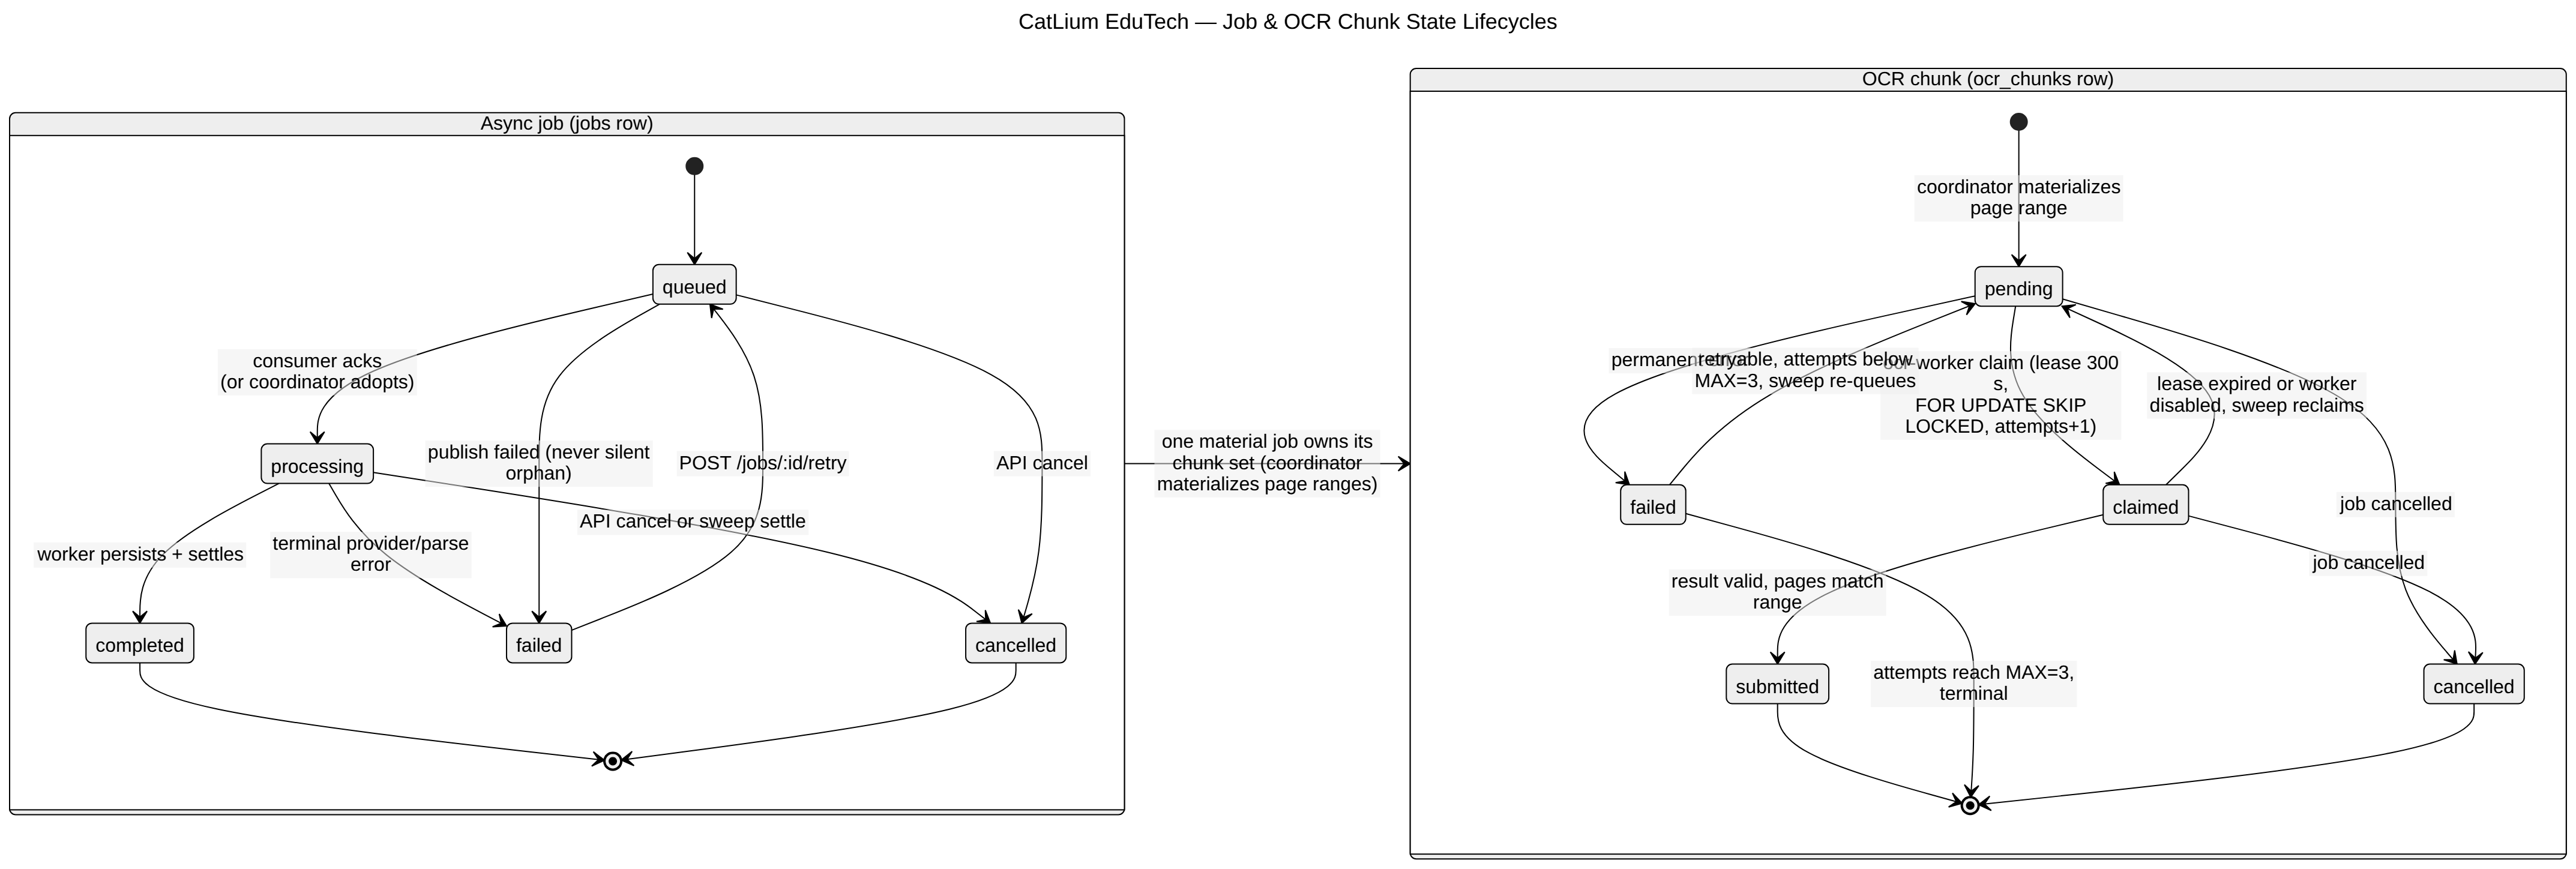
\includegraphics[width=\textwidth]{figures/ocr-chunk-state-bw.png}
\caption{Job and OCR chunk state lifecycles.}
\label{fig:ocrstate}
\end{figure}

\subsection{AI generation}

AI generation is asynchronous and validated at both ends. The API publishes
a generation job; the AI worker chunks large sources, calls the internal
OpenAI-compatible gateway through OmniRoute, validates each chunk's output
against canonical schemas, re-requests on validation failure, aggregates the
results deterministically, and persists them; the client polls job status.
Figure~\ref{fig:ai} shows the sequence.

\begin{figure}[H]
\centering
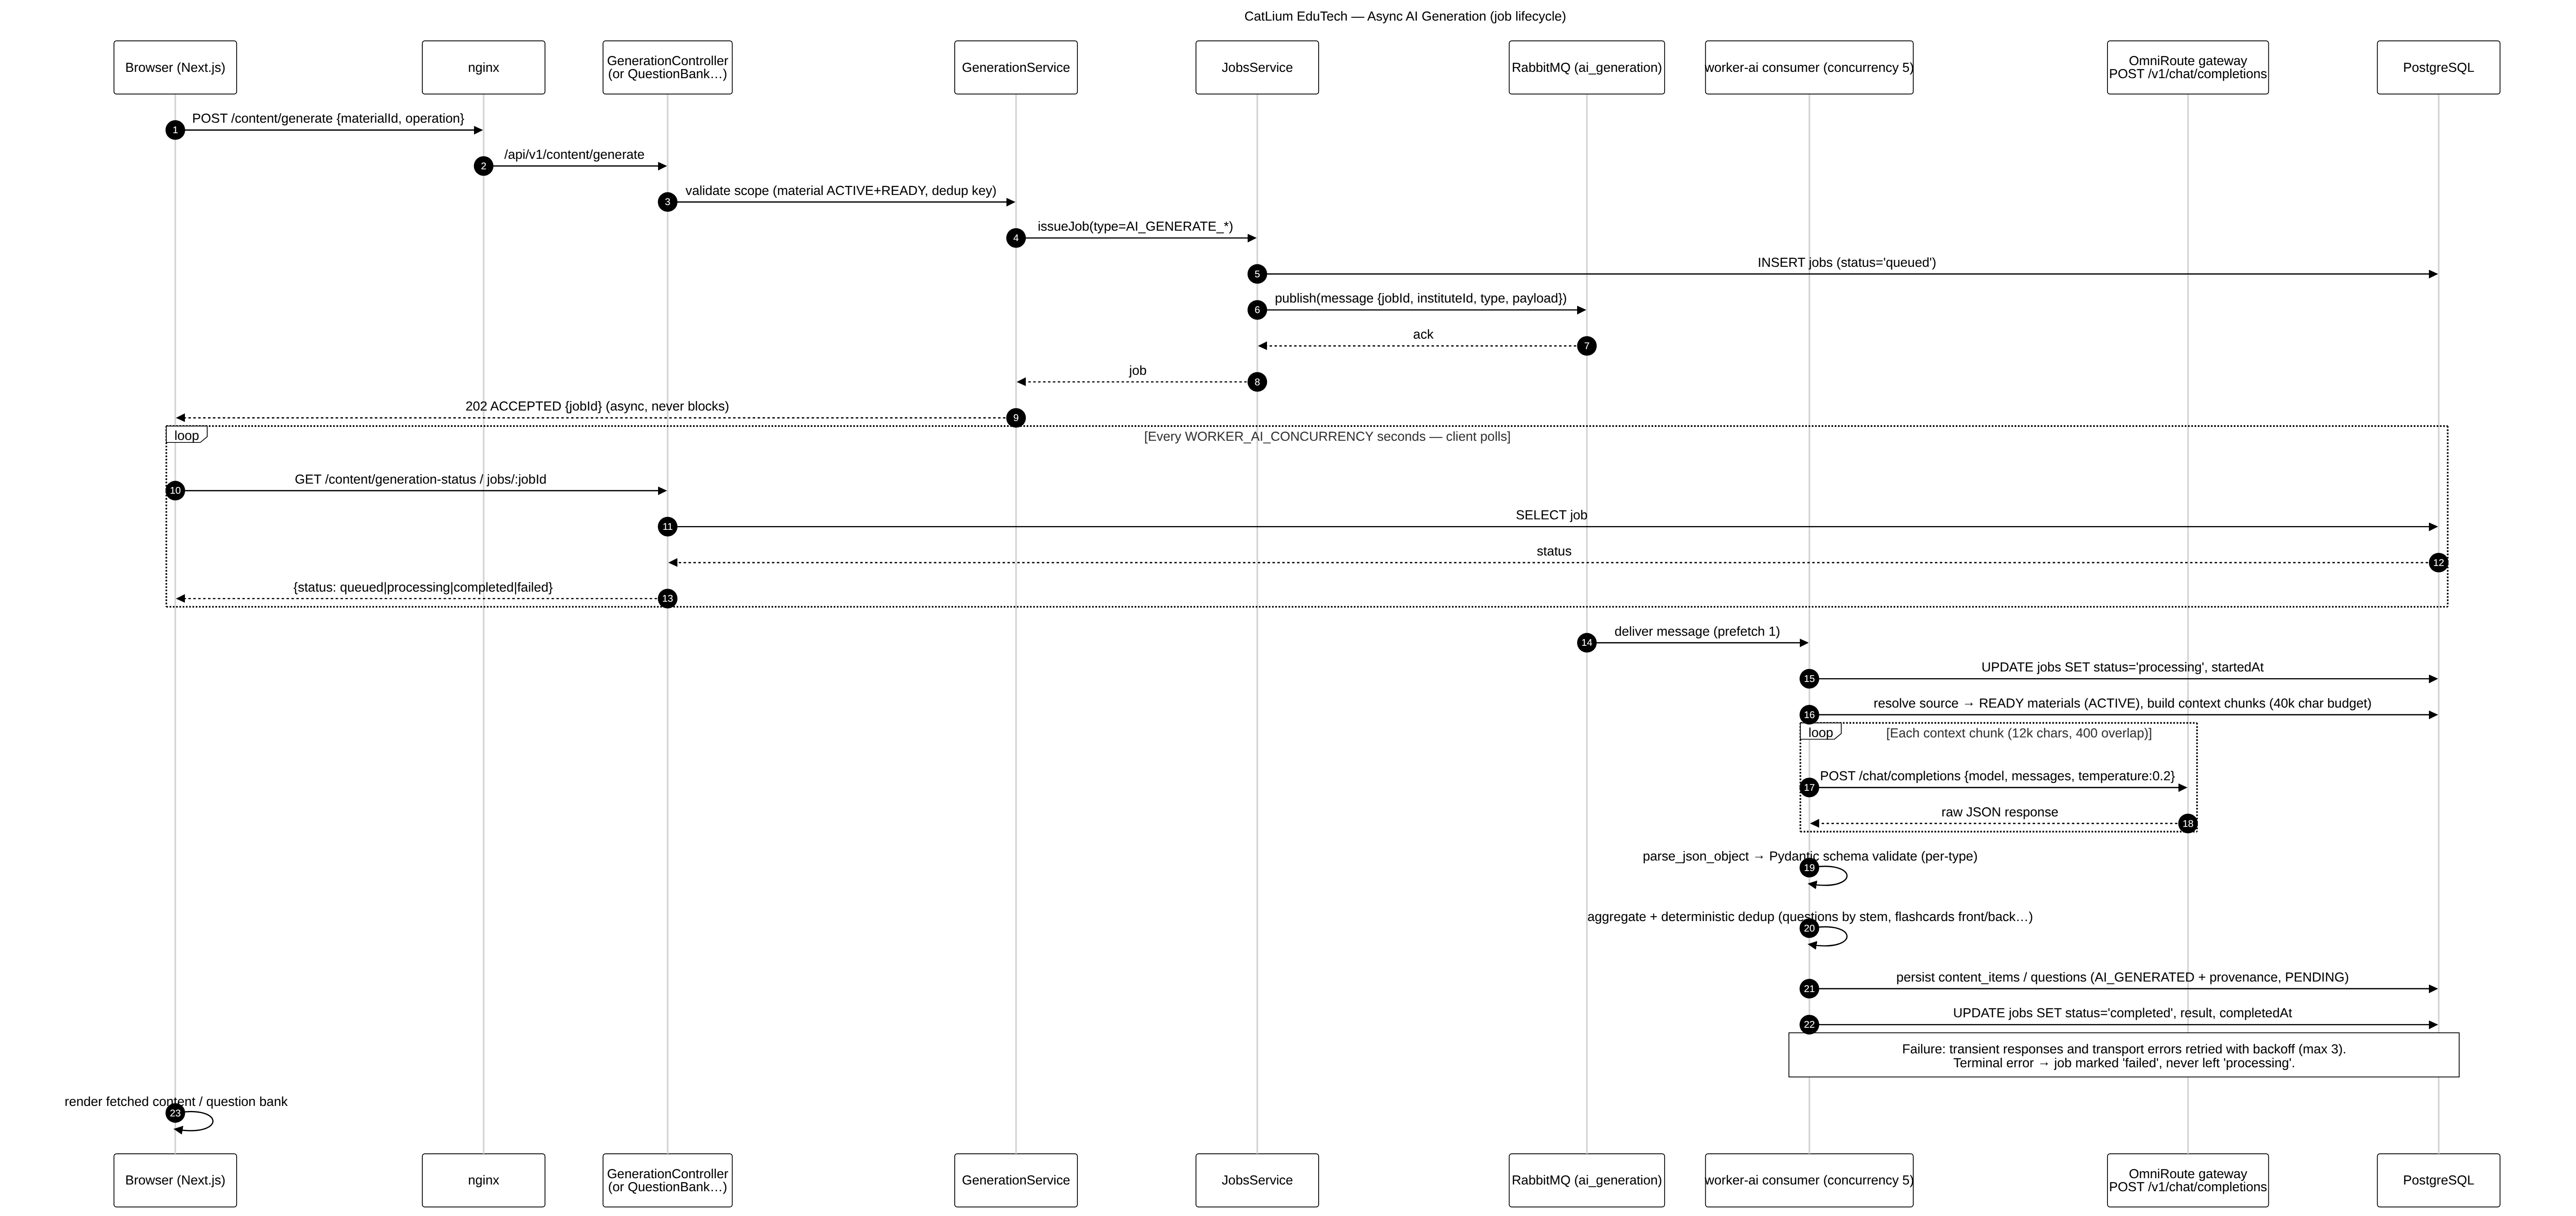
\includegraphics[width=\textwidth]{figures/ai-generation-sequence-bw.png}
\caption{Asynchronous AI generation sequence.}
\label{fig:ai}
\end{figure}